\documentclass[tikz,border=2pt]{standalone}
\usepackage{amsmath}
\usepackage{pgfplots}
\pgfplotsset{compat=1.18}
\usetikzlibrary{arrows.meta}
\begin{document}
% Example 1.3: V={(2,1),(1,1),(3,-1),(-3,-4),(-2,0),(0,5)}; Conv(V) is the quadrilateral with corners (0,5),(3,-1),(-3,-4),(-2,0);
% (2,1)=(1/3)(0,5)+(2/3)(3,-1) lies on an edge, (1,1)=(2/5)(0,5)+(7/15)(3,-1)+(2/15)(-3,-4) lies inside.
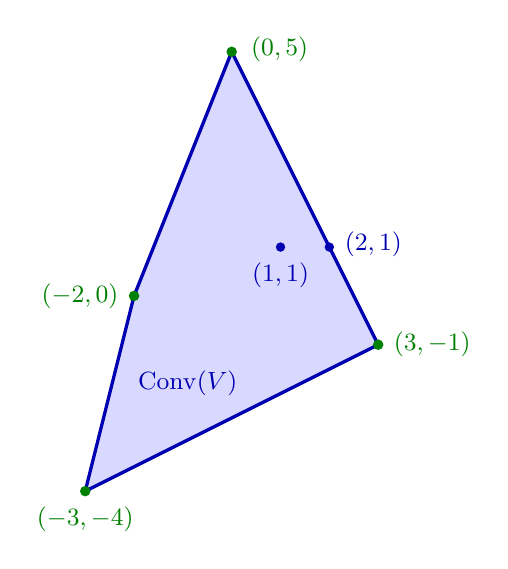
\begin{tikzpicture}[font=\small, >={Latex[length=2mm]}, x=0.62cm, y=0.62cm]
  \fill[blue!15] (0,5) -- (3,-1) -- (-3,-4) -- (-2,0) -- cycle;
  \draw[blue!70!black, very thick] (0,5) -- (3,-1) -- (-3,-4) -- (-2,0) -- cycle;
  \foreach \p in {(0,5),(3,-1),(-3,-4),(-2,0)} \fill[green!50!black] \p circle (1.9pt);
  \fill[blue!70!black] (2,1) circle (1.7pt);
  \fill[blue!70!black] (1,1) circle (1.7pt);
  \node[green!50!black, anchor=west] at (0.2,5.05) {$(0,5)$};
  \node[green!50!black, anchor=west] at (3.12,-1) {$(3,-1)$};
  \node[green!50!black, anchor=north] at (-3,-4.12) {$(-3,-4)$};
  \node[green!50!black, anchor=east] at (-2.12,0) {$(-2,0)$};
  \node[blue!70!black, anchor=west] at (2.12,1.05) {$(2,1)$};
  \node[blue!70!black, anchor=north] at (1,0.88) {$(1,1)$};
  \node[blue!70!black] at (-0.9,-1.8) {$\operatorname{Conv}(V)$};
\end{tikzpicture}
\end{document}
